%General Lab Training
% Updated 2/11/2017

\chapter{General Lab Safety}

This chapter will cover basic tools and general information of the 0620 Lab Space also known as the M:2:I Lab  This document will cover some of the basic lab rules, procedures and information that all students should know in order to use the lab.  It will also cover some of the basic tools available to students.  Students should take the M:2:I General Lab Quiz on blackboard after they have read this training.

\section{Introduction}

The Make to Innovate Lab space offers a number of equipment and services that are available to students to use while working on their Make to Innovate (M:2:I) projects.  This includes the following:

\begin{itemize}
\item Electrical construction and diagnostic
\item Basic metal working
\item Basic wood working
\item Foam cutting and shaping tools
\item 3D Printers
\item Tabletop CNC machine
\end{itemize}

These tools and equipment are only accessible to students that are currently enrolled in the Make to Innovate program and currently assigned to an active and authorized project within M:2:I.  All other students must receive written permission from the M:2:I Program Coordinator.

Not all equipment in the lab can be used by students.  Some equipment, such as the 3D printers, and CNC machine can only be used by an authorized personnel.  Contact a lab monitor or the program coordinator if you need to use this equipment.  Additional costs may apply and can be charged to your project account.

Students wishing to use the 0620 lab space and any of the tools in the space must complete the following training:

\begin{enumerate}
\item Fire Safety and Extinguisher Training course
\item Personal Protective Equipment course
\item M:2:I General Lab Training
\end{enumerate}

Optionally students may take the EH\&S Shop Safety training.  This training provides some basics on shop safety and usage of tools.  However, the M:2:I General Lab Training will also cover many of the same things covered by the EH\&S Shop Safety Training.

These EH\&S training courses can be found at \url{http://www.ehs.iastate.edu/my-eh-s/training}. From there, click on ISU Login and enter your Iowa State login information. Then navigate to the Course Catalog page, which can be found on the left hand side bar. Type in the course name and click the Launch button to take the training. When completed, bring a printed copy of your completion certificates to the lab monitor on duty.  If you have a problem with the EH\&S website, please contact EH\&S.

Additional training may also be required in order to use certain tools and lab equipment.  Use of the electronics bench and foam cutter both require additional training and a quiz that needs to be passed by the student.  The foam cutter training can be found in Chapter \ref{foam_training} and the basic electronics training can be found in Chapter \ref{basic_electronics}.

\section{Hazards}
While we have taken many precautions to make the M:2:I Lab as safe as possible, students must still be aware that there are hazards in the lab.  With the proper training, personal protection equipment and care these hazards can be minimized and the impact to the student should be small.  However, students must always be aware that these hazards exist.  

\subsection{Electrocution}
\begin{framed}
\begin{wrapfigure}{L}{0.15\linewidth}
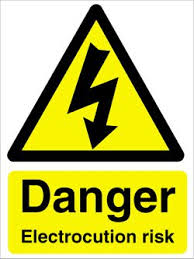
\includegraphics[width=\linewidth]{images/electrocution_hazard.jpg}
\end{wrapfigure}
\ \\
This lab space offers tools used for electrical testing and prototyping as well as power tools. All of these can potentially cause electrocution if improperly used. When using electrical equipment with power cords, always inspect the cords for damage prior to use. Never attempt to repair a damaged cord.
\end{framed}
Report any damaged cord or potential hazard to a lab monitor immediately. Never use a cord that is frayed or damaged as this can lead to electrocution.  Always ensure that when plugging in equipment, the plug is fully inserted into the outlet and has a snug fit. If the plug is equipped with a ground plug, the plug must still be in tact and must not be damaged.  Cords that aren't securely plugged in present a potential electrocution hazard. 

Extension cords may only be used for \emph{temporary} use.  Extension cords must be rated for the amperage the equipment requires.  Power strips may not be used for any power tool.  Use of power strips for low power applications is permitted.  When using tools or instruments that have specific training requirements, always complete the training and familiarize yourself with the operating procedures to reduce the risk of shock.

The electrical workbench has several bench power supplies that can supply both high voltage and high current.  Proper precautions must be observed to ensure to minimize risk to the user.  Additional information on the power supplies will be covered in Section \ref{power_supply}

\subsection{Burns}
\begin{framed}
\begin{wrapfigure}{L}{0.15\linewidth}
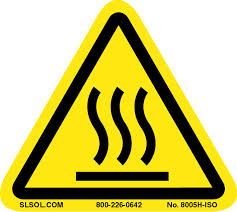
\includegraphics[width=\linewidth]{images/burn_hazard.jpg}
\end{wrapfigure}
Several tools in this lab space utilize heat in order to perform their designated task. Wearing gloves that are heat resistant when handling hot objects will help to reduce the risk of burns. Always be familiar with the safety and operating procedures of the tool being used in order to minimize burn risks. 
\end{framed}
Always be aware of your surroundings and others while working with hot tools and materials. If you are unsure how to use a tool, seek help from a lab monitor.  Some tools, such as the soldering irons, require additional training as well.

\subsection{Fumes}
\begin{framed}
\begin{wrapfigure}{L}{0.16\linewidth}
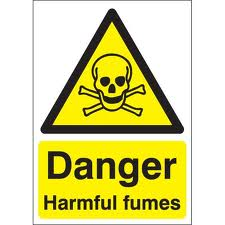
\includegraphics[width=\linewidth]{images/fumes_hazard.jpg}
\end{wrapfigure}
\ \\
Fumes may be present in this lab space. The most common sources will be from soldering and the various chemicals being used in the lab such as adhesives. Fumes have the potential to cause respiratory and ocular damage if not properly managed. Always read chemical labels before use. Always use a vent hood when dealing with volatile chemicals or items that can cause harmful fumes.
\end{framed}

Students must wear the appropriate PPE equipment when working with any chemical that poses a health risk.  If at any time you are uncertain what PPE should be worn, either consult with the MSDS sheets for that chemical or talk to a Lab Monitor or the Program Coordinator.  

\subsection{Chemicals}
Several chemicals may be in use in the lab and chemicals have the potential to cause injury from mild skin and eye irritation to severe burns and potentially death. In order to minimize this risk, be familiar with the chemical prior to use. Read and follow all safety information listed on the chemical. Always use a proper vent hood when dealing with chemicals that create harmful fumes.  Proper PPE equipment must also always be used when appropriate.  

\subsection{Cuts}
\begin{framed}
\begin{wrapfigure}{L}{0.15\linewidth}
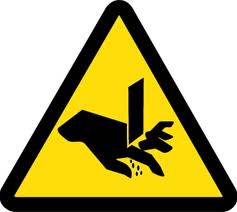
\includegraphics[width=\linewidth]{images/cut_hazard.jpg}
\end{wrapfigure}
\ \\
Many of the tools in the lab can lead to cuts, both minor and severe if improperly used. Having the appropriate training that each tool requires is the best way to minimize the risk of cuts. 
\end{framed}
Always make sure that your immediate surroundings is cleared of potential hazards and other people before using cutting tools as this helps reduce the risk of injury to both yourself and others. Always cut away from yourself and bystanders. Don’t wear loose fitting clothing as this can be caught in the cutting tool and cause injury. 

\section{Safety}
Safety is our top concern in the Make to Innovate lab.  We want our students to be able to work on their projects in a safe and clean environment.  Because of this, we require all students to take the EH\&S trainings that cover personal protection equipment and fire safety and the M:2:I General Lab Training.  These courses contain a majority of the basic safety measures for the lab space and is often a requirement for other lab spaces on the campus of ISU. Addition signs have also been placed within the lab that relates to a specific risk or PPE that must be worn.  Read and become familiar with these regulations. 

There are two First aid kits in the lab that can address minor cuts, burns and irritations.  You should become familiar with the locations of these kits. Fire extinguishers are also near the exits of the lab and near the electronics area. Please refer to Figure \ref{fig:0620_floor_plan} that has a map of key safety features of the lab.

\subsection{Basic Safety Rules}
The lab has a set of basic safety rules that all students, faculty, staff and visitors should know.  All of these rules are also posted in the lab to remind everyone and inform visitors on these basic rules.  The following is the basic safety information that all persons in the lab need to know.

\begin{itemize}
\item No open sole shoes are allowed at any time
\item No loose jewelry or clothing is allowed at any time
\item Long pants must be worn at all times
\item Safety glasses must be worn in all designated areas
\item All signs posted must be adhered to at all times
\item Long hair must be securely pulled back
\end{itemize}

These basic rules apply to all those in the lab.  This includes all M:2:I students, faculty and staff and all visitors to the lab space.  If a person is caught that is not following theses rules, they will be asked to leave the lab or correct the error.

\section{Emergency procedures}
It is important to know the emergency procedures of the lab.  The lab has this information posted on signs near the exits of the lab as well as the evacuation routes.  A copy of this sign is also shown in Figure \ref{fig:Emergency_Response}. Please note that 0620 is also a tornado shelter in the event of a tornado.  In addition to the emergency signs, you need to familiarize yourself with the following.
\begin{itemize}
\item Know where all safety signs and emergency information is in the lab,
\item Know where all safety equipment is located,
\item Know the location of the fire extinguishers and first aid kits in the lab
\end{itemize}

\begin{figure}[ht]
\centering
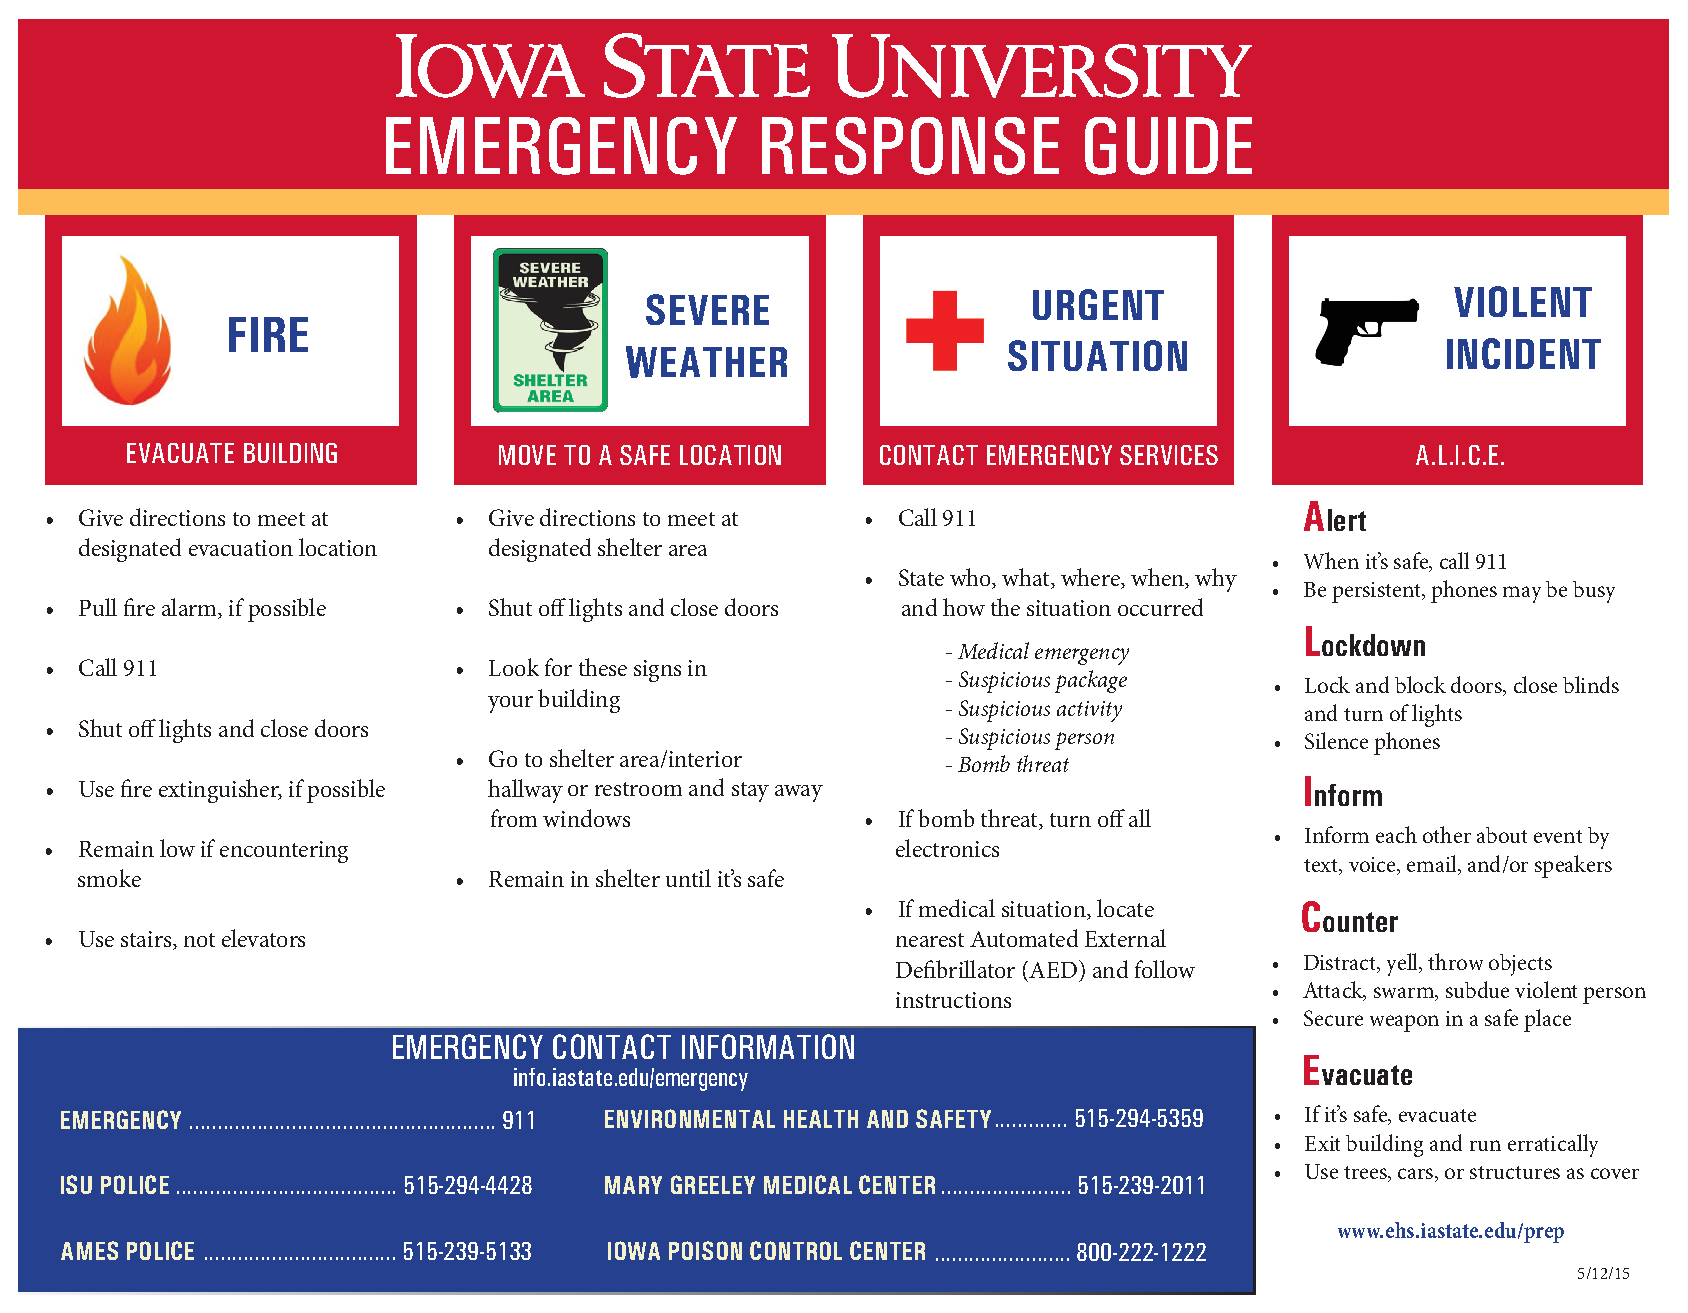
\includegraphics[width=6in]{images/EmergencyPoster.pdf}
\caption{ISU Emergency Response Guide Poster}
\label{fig:Emergency_Response}
\end{figure}

\subsection{Emergency Evacuation and Procedures}
In the event of a fire or other emergency students will be asked to leave Howe Hall in a safe and orderly manor.  Personnel should evacuate using the route indicated in Figure \ref{fig:Evac_map}.  In the event that the fire alarm has been activated, all personnel must evacuate the building immediately as per Iowa Law and ISU policy.  Even if it is suspected the alarm might be false, everyone must evacuate.  The building is only safe to return to when emergency responders have deemed it safe to enter the building again.

\begin{figure}[ht]
\centering
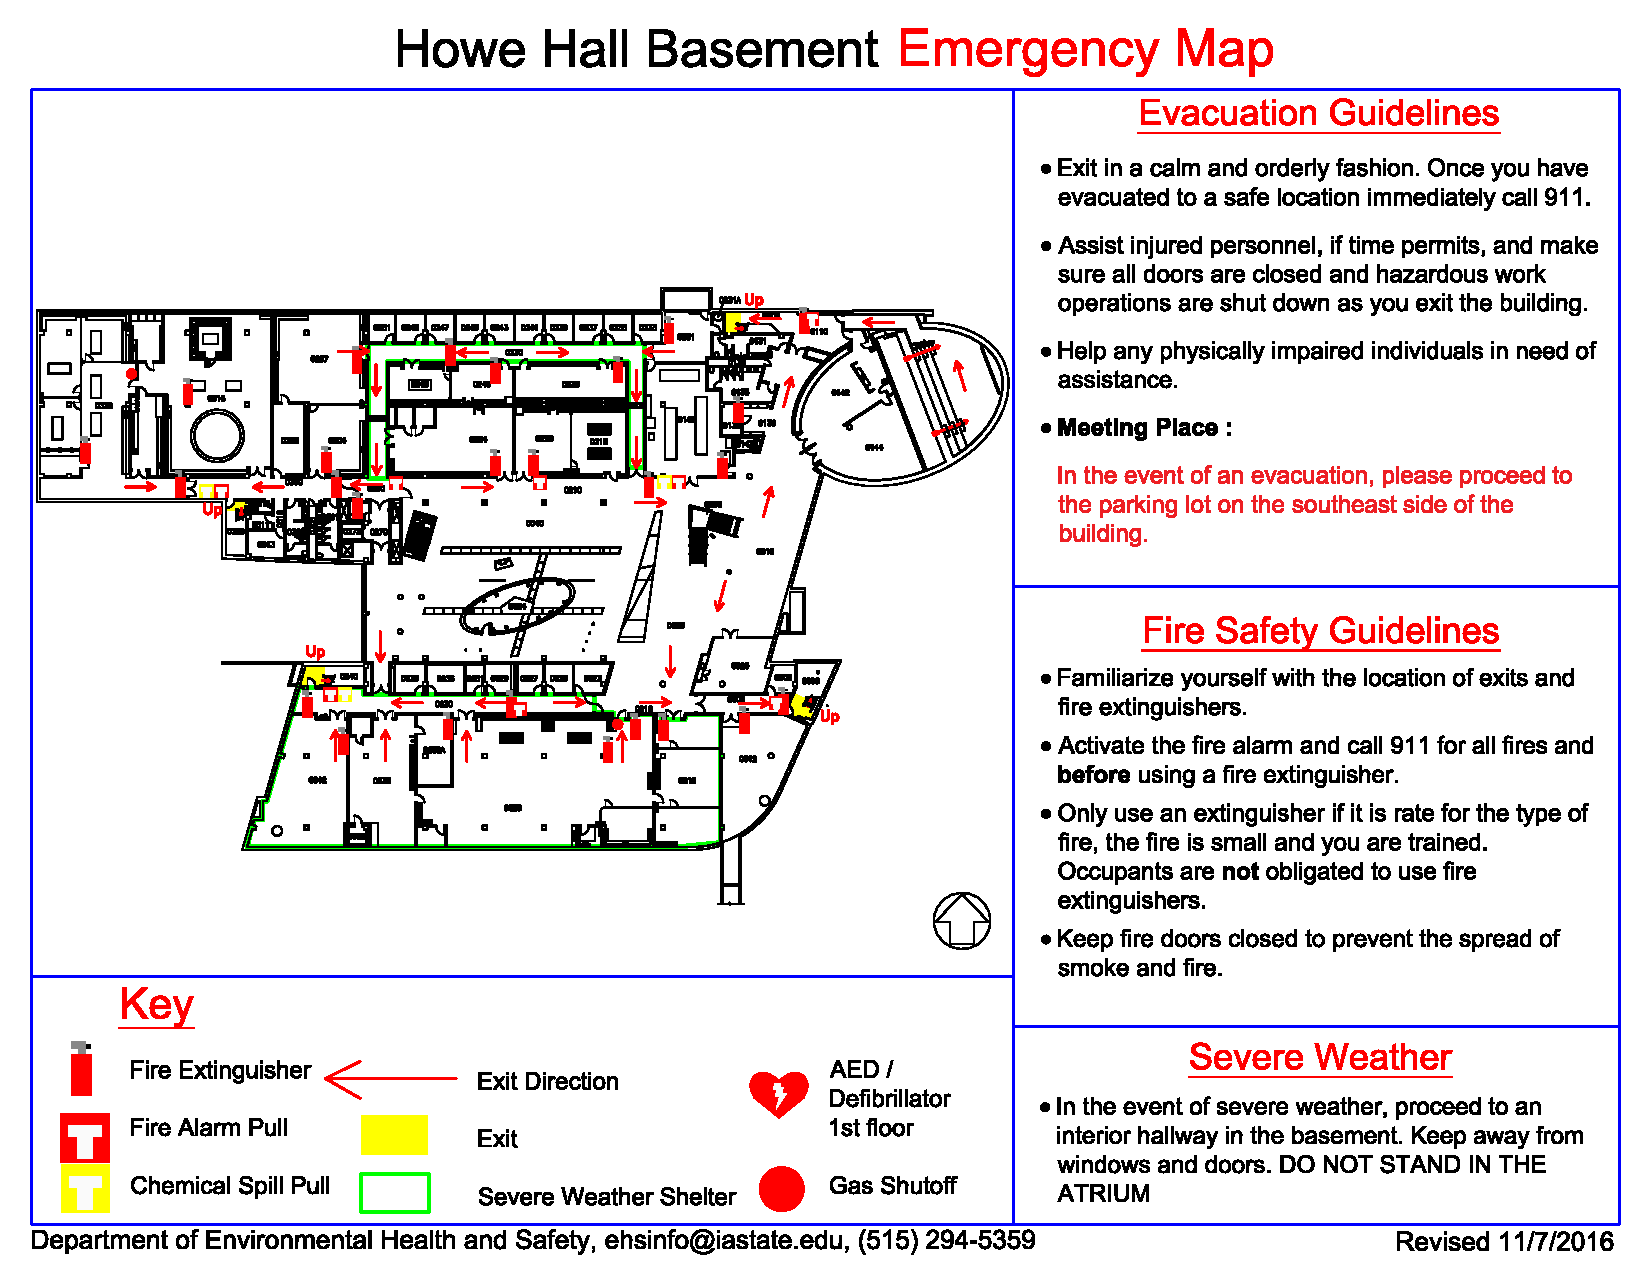
\includegraphics[width=6in]{Howe-Bsmt.pdf}
\caption{Howe Hall Evacuation Map}
\label{fig:Evac_map}
\end{figure}

The 0620 Lab Space is a designated tornado shelter and personnel may remain in the lab during severe weather.  In the event of a tornado all personnel should stay in the lab or in the most inner room of the lab.  Those spaces are 0620A, 0620B and 0620E within the lab space.

\chapter{Lab Facilities}
The lab has facilities that can be used by students for their projects.  This includes storage of their project materials, a conference room as well as additional storage for raw materials.  The lab also has work tables, work benches that projects can use for assembly and construction work on their projects.  Finally, the lab has several pieces of equipment that are used for design and construction such as a drill press, CNC machine, down draft table and computer lab.

\begin{figure}[ht]
\centering
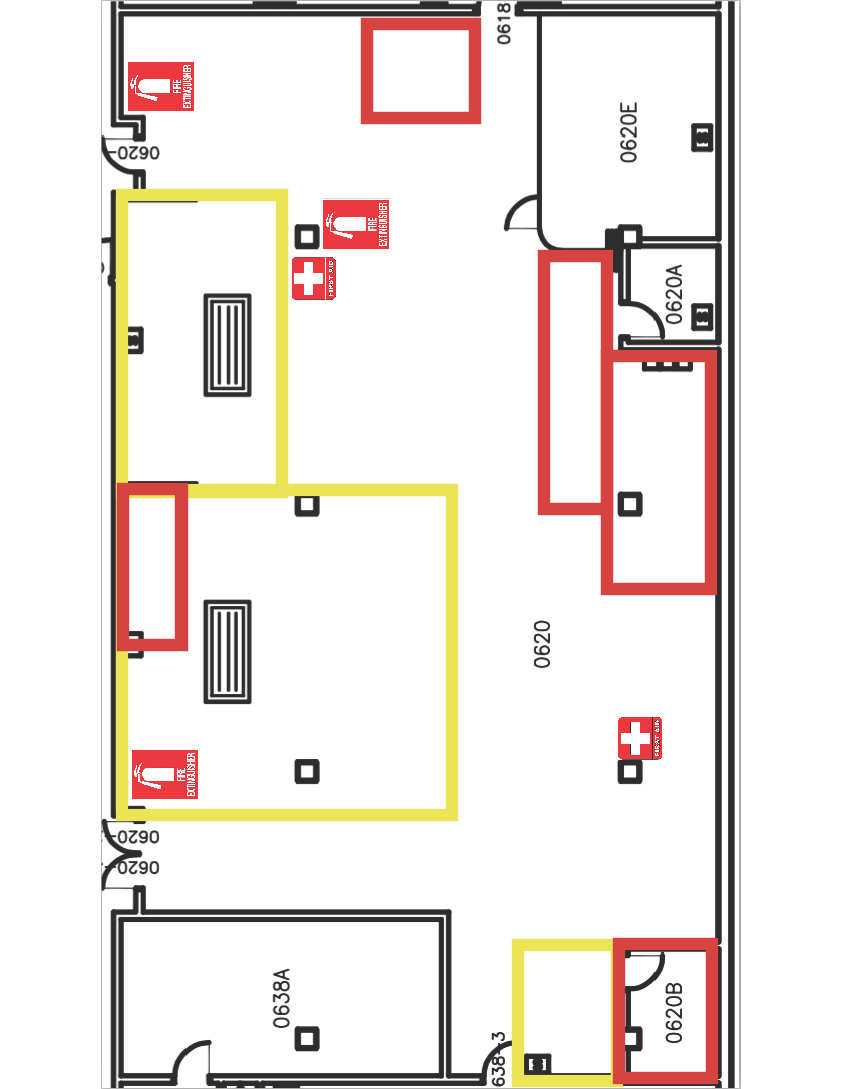
\includegraphics[width=5.8in]{images/0620_Floor_Plan.png}
\caption{0620 Floor plan with safety glasses (yellow), first aid, fire extinguishers, and restricted areas (red) marked}
\label{fig:0620_floor_plan}
\end{figure}

The M:2:I Lab has a fairly open concept and as such we have equipment that is often used that can generate hazards.  The lab has been organized to keep hazardous equipment in one area so that other areas may be used for less hazardous work.  Figure \ref{fig:0620_floor_plan} shows a floor plan of the lab with areas marked that are restricted or require safety glasses at all times.  Areas in yellow require safety glasses safety glasses at all times.  Areas in red are restricted to only M:2:I faculty, staff, lab monitors and lab technicians.  No students are permitted in these areas at any time.

\section{Project Storage Lockers}
The M:2:I Lab has storage lockers that projects can use to store their equipment, work in progress and finished parts.  The M:2:I Lab has full size lockers, smaller storage drawers and storage shelves to hold a variety of sizes of equipment and parts.  All M:2:I projects must be assigned these spaces.  If a project requires more space than what is currently available, they should talk to the M:2:I Program Coordinator.

\section{Storage Room}
The storage room is located in 0620B and contains building materials such as foam and wood. It also has spare parts from previous projects such as motors, servos, props and other smaller equipment.  Projects are free to use this material. In order to do so, groups must first seek out a lab monitor, who will open the room.  Lab monitors will keep track of the rough quantity that each group is using of each material. This will ensure that a groups are not using an excessive amount of materials. The storage room is for lab storage only; unauthorized objects will be jailed or requisitioned for lab supplies. Only under special circumstances will a group be allowed to store material in the storage room. This requires the approval of the M:2:I Program Coordinator.

If a project requires a large purchasing of materials and to have that stored, they must request the materials be ordered and must have permission of the M:2:I Program Coordinator to store items in the storage room.  Projects may have the items charged to their account.  This will be at the discretion of the M:2:I Program Coordinator.  

\section{Supply Room}
The supply room, located in 0620A, contains various cleaning materials and office supplies. This room is restricted to lab monitors and M:2:I faculty and staff only. If paper towels, markers, or any other related items run out, tell a lab monitor and they will take care of replacing the items in question. The supply room is strictly for lab use only and will not be used to store any project related materials.

\section{Conference Room}
The lab conference room is a space that has been set aside for use by M2I groups and for the Aerospace Engineering Department. Projects may request to use the conference room for project or team meetings.  In order to request using the conference room, you must email the M:2:I Program Coordinator.  A calendar will be kept near the Lab Monitors desk.

\section{Computer Lab Area}
The computer lab area houses 10 Dell computers running Windows 10 and a variety of software.  Software that is normally available to Engineering students such as Matlab, Solid Works, LabView, Microsoft Office, and others are installed on these machines.  In addition to these machines, the M:2:I Lab also has 24 Dell laptops that may be checked out for short durations.  

\section{3D Printing Area}
The 3D Printing Area is a restricted area that only authorized personnel are permitted in.  This area has the 5 3D printers that are used for both M:2:I and other projects.  If a M:2:I project wishes to print something on the 3D printers, they should contact the M:2:I Program Coordinator or Christine Nelson in 1200 Howe Hall.

